\documentclass[../main/main.tex]{subfiles}

\newdate{date}{02}{12}{2020}

% \begin{figure}[h!]
% \centering
% \includegraphics[page=6,width=0.8\textwidth]{../lessons/pdf_file/22_lecture.pdf}
% \end{figure}

%\displaydate{date}. Compiled:  \today. Alice.

\begin{document}

\pagestyle{plain}

\section{Lecture 22}


\subsubsection*{Slide 1}

\begin{minipage}[]{0.5\linewidth}
\centering
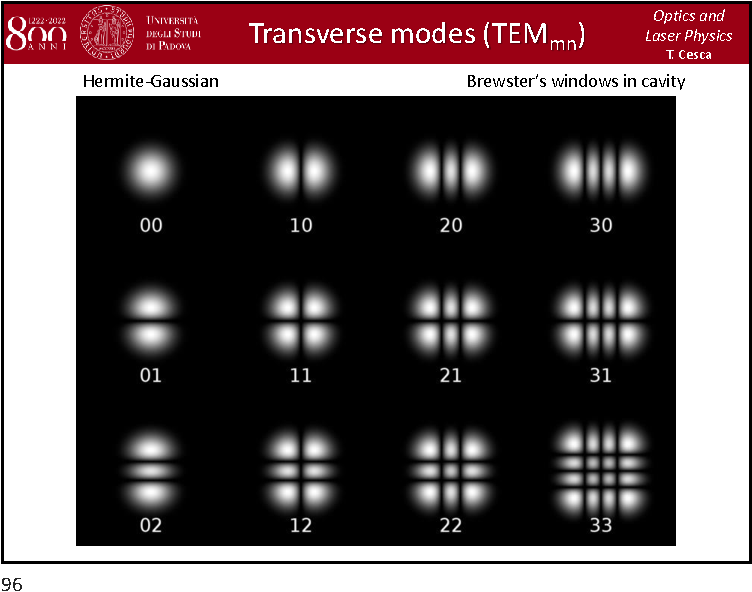
\includegraphics[page=1,width=1\textwidth]{../lessons/pdf_file/22_lecture.pdf}
\end{minipage}
\hspace{0.3cm}\vspace{0.3cm}
\begin{minipage}[c]{0.47\linewidth}

Let us see how the property of the cavity control the properties of the beam. These are simulation for transverse modes.

\end{minipage}

\subsubsection*{Slide 2}

\begin{minipage}[]{0.5\linewidth}
\centering
\includegraphics[page=2,width=1\textwidth]{../lessons/pdf_file/22_lecture.pdf}
\end{minipage}
\hspace{0.3cm}\vspace{0.3cm}
\begin{minipage}[c]{0.47\linewidth}

This is the expression of the electromagnetic field.

\end{minipage}

\subsubsection*{Slide 3}

\begin{minipage}[]{0.5\linewidth}
\centering
\includegraphics[page=3,width=1\textwidth]{../lessons/pdf_file/22_lecture.pdf}
\end{minipage}
\hspace{0.3cm}\vspace{0.3cm}
\begin{minipage}[c]{0.47\linewidth}

It is controlled by these main paramaters.

At \( w_0 \) the radius of curvature is infinite.

\end{minipage}

\newpage

\subsubsection*{Slide 4}

\begin{minipage}[]{0.5\linewidth}
\centering
\includegraphics[page=4,width=1\textwidth]{../lessons/pdf_file/22_lecture.pdf}
\end{minipage}
\hspace{0.3cm}\vspace{0.3cm}
\begin{minipage}[c]{0.47\linewidth}

Let us see how we can determien the properties starting from the characterstic of the cavity. Let us consider a symmetric two-mirror optical cavity.

\( R(z) \) is the curvature radius of the electromagnetic field.

The wavefront at the position of the mirror has to be equal to the radius of the mirror!

If we make the calculation we have an expression for the radius of curvature. We can reverse the expression for the Rayleigh range of the beam.

We have imposed \( R(z = d/2)  = R\)!

They control the characteristic of the beam also outside the cavity.

\end{minipage}

\subsubsection*{Slide 5}

\begin{minipage}[]{0.5\linewidth}
\centering
\includegraphics[page=5,width=1\textwidth]{../lessons/pdf_file/22_lecture.pdf}
\end{minipage}
\hspace{0.3cm}\vspace{0.3cm}
\begin{minipage}[c]{0.47\linewidth}

Let us consider a \textbf{confocal resonator}. The focal point of the two mirror is the same and its at the center of the cavity.

We obtain that the Rayleigh range is half the distance between the two mirrors.

Once you have the beam waist you wan compute the beam spot radius at any position \( z \).

\end{minipage}

\subsubsection*{Slide 6}

\begin{minipage}[]{0.5\linewidth}
\centering
\includegraphics[page=6,width=1\textwidth]{../lessons/pdf_file/22_lecture.pdf}
\end{minipage}
\hspace{0.3cm}\vspace{0.3cm}
\begin{minipage}[c]{0.47\linewidth}

Just to have some realistic numbers.

We can also calculate the \textbf{far-field beam divergence}. We have a very small divergence, that is why we image a laser beam as a collimated beam!

\end{minipage}

\newpage

\subsubsection*{Slide 7}

\begin{minipage}[]{0.5\linewidth}
\centering
\includegraphics[page=7,width=1\textwidth]{../lessons/pdf_file/22_lecture.pdf}
\end{minipage}
\hspace{0.3cm}\vspace{0.3cm}
\begin{minipage}[c]{0.47\linewidth}

Let us consider an \textbf{asymmetrical cavity}. We want to determine the parameters of the beam from this cavity with two mirror with different radii of curvature.

We have to determine where is the zero for this system of reference. It is easy if we apply the sign convention which we said at the beginning. We have the \( z \) axis which is the propagation axis. We think that we are no more inside the cavity, but the light comes from the left and go to the right.

Let us suppose that the zero is placed here.

We have to impose the boundary conditions. The radius of curvature at the two points \( z_1 \) and \( z_2 \) has to be equal to \( R \).

We have three unkwown paramaters: \( z_0 \), \( z_1 \) and \( z_2 \).

\end{minipage}

\subsubsection*{Slide 8}

\begin{minipage}[]{0.5\linewidth}
\centering
\includegraphics[page=8,width=1\textwidth]{../lessons/pdf_file/22_lecture.pdf}
\end{minipage}
\hspace{0.3cm}\vspace{0.3cm}
\begin{minipage}[c]{0.47\linewidth}

We obtain an expression for the Rayleigh range \( z_0 \).

We determine also \( z_2 \) given the two radii of curvature. Hence, we known where is the zero of the coordinate of reference.

\end{minipage}

\subsubsection*{Slide 9}

\begin{minipage}[]{0.5\linewidth}
\centering
\includegraphics[page=9,width=1\textwidth]{../lessons/pdf_file/22_lecture.pdf}
\end{minipage}
\hspace{0.3cm}\vspace{0.3cm}
\begin{minipage}[c]{0.47\linewidth}

Once we have determined \( z_2 \), we have determined all the important parameters.

If \( z_0 \) is a real number, the cavity is a \textbf{stable cavity}. If \( z_0 \) is a complex number, the cavity is \textbf{unstable}.

\end{minipage}

\subsubsection*{Slide 10}

\begin{minipage}[]{0.5\linewidth}
\centering
\includegraphics[page=10,width=1\textwidth]{../lessons/pdf_file/22_lecture.pdf}
\end{minipage}
\hspace{0.3cm}\vspace{0.3cm}
\begin{minipage}[c]{0.47\linewidth}

If one of the two mirrors is a plane, the beam waist will be at the plane mirror.

\end{minipage}

\subsubsection*{Slide 11}

\begin{minipage}[]{0.5\linewidth}
\centering
\includegraphics[page=11,width=1\textwidth]{../lessons/pdf_file/22_lecture.pdf}
\end{minipage}
\hspace{0.3cm}\vspace{0.3cm}
\begin{minipage}[c]{0.47\linewidth}

Let us make an example.

\end{minipage}

\subsubsection*{Slide 12}

\begin{minipage}[]{0.5\linewidth}
\centering
\includegraphics[page=12,width=1\textwidth]{../lessons/pdf_file/22_lecture.pdf}
\end{minipage}
\hspace{0.3cm}\vspace{0.3cm}
\begin{minipage}[c]{0.47\linewidth}

\end{minipage}

\subsubsection*{Slide 13}

\begin{minipage}[]{0.5\linewidth}
\centering
\includegraphics[page=13,width=1\textwidth]{../lessons/pdf_file/22_lecture.pdf}
\end{minipage}
\hspace{0.3cm}\vspace{0.3cm}
\begin{minipage}[c]{0.47\linewidth}

\end{minipage}

\subsubsection*{Slide 14}

\begin{minipage}[]{0.5\linewidth}
\centering
\includegraphics[page=14,width=1\textwidth]{../lessons/pdf_file/22_lecture.pdf}
\end{minipage}
\hspace{0.3cm}\vspace{0.3cm}
\begin{minipage}[c]{0.47\linewidth}

Once we have the beam waist and the curvature radius in one specific point, we can determinine for every point.

We have just to set \( R(z) = R \).

\end{minipage}

\subsubsection*{Slide 15}

\begin{minipage}[]{0.5\linewidth}
\centering
\includegraphics[page=15,width=1\textwidth]{../lessons/pdf_file/22_lecture.pdf}
\end{minipage}
\hspace{0.3cm}\vspace{0.3cm}
\begin{minipage}[c]{0.47\linewidth}

Let us see what happens when a Gaussian beam is interacting with optical elements. The propagation of a Gaussian beam trough any optical element is different from what we have seen in geometrical optics. We have a techniques which allows us to calculate the propagation of a Gaussian beam trough any optical element if we know the ABCD matrix of the optical elements.

We have to introduce the \textbf{complex parameter} of the Gaussian beam.

\end{minipage}

\subsubsection*{Slide 16}

\begin{minipage}[]{0.5\linewidth}
\centering
\includegraphics[page=16,width=1\textwidth]{../lessons/pdf_file/22_lecture.pdf}
\end{minipage}
\hspace{0.3cm}\vspace{0.3cm}
\begin{minipage}[c]{0.47\linewidth}

Consider that \( at z=0 \) we have \( R(z) = \infty  \), the complex parameter at \( z=0 \) as a simple expression.

\( q(z) \) is the \textbf{complex curvature radius} of the Gaussian beam. It transfor itself as the curvature radius of a spherical wave.

\end{minipage}

\subsubsection*{Slide 17}

\begin{minipage}[]{0.5\linewidth}
\centering
\includegraphics[page=17,width=1\textwidth]{../lessons/pdf_file/22_lecture.pdf}
\end{minipage}
\hspace{0.3cm}\vspace{0.3cm}
\begin{minipage}[c]{0.47\linewidth}

How this complex parameter can tell us? We do not demonstrate these results.

Let us consider the free-space propagation (this is our optical element).

\end{minipage}

\subsubsection*{Slide 18}

\begin{minipage}[]{0.5\linewidth}
\centering
\includegraphics[page=18,width=1\textwidth]{../lessons/pdf_file/22_lecture.pdf}
\end{minipage}
\hspace{0.3cm}\vspace{0.3cm}
\begin{minipage}[c]{0.47\linewidth}

We obtain the same results that we already knew by appling propagation relation!

\end{minipage}

\subsubsection*{Slide 19}

\begin{minipage}[]{0.5\linewidth}
\centering
\includegraphics[page=19,width=1\textwidth]{../lessons/pdf_file/22_lecture.pdf}
\end{minipage}
\hspace{0.3cm}\vspace{0.3cm}
\begin{minipage}[c]{0.47\linewidth}

Let us assume a Gaussian beam with a plane wavefront which is impinging on a thin lens. We will have the propagation after the interaction.

Our optical system is the lens and the propagation after the lens.

\end{minipage}

\subsubsection*{Slide 20}

\begin{minipage}[]{0.5\linewidth}
\centering
\includegraphics[page=20,width=1\textwidth]{../lessons/pdf_file/22_lecture.pdf}
\end{minipage}
\hspace{0.3cm}\vspace{0.3cm}
\begin{minipage}[c]{0.47\linewidth}

\( z_{min} \) is when the radius of curvature is infinite after the interaction with the lens.

\end{minipage}

\subsubsection*{Slide 21}

\begin{minipage}[]{0.5\linewidth}
\centering
\includegraphics[page=21,width=1\textwidth]{../lessons/pdf_file/22_lecture.pdf}
\end{minipage}
\hspace{0.3cm}\vspace{0.3cm}
\begin{minipage}[c]{0.47\linewidth}

In principle \( z_{min} \) is smaller than the focal length!
It will be focalized in principle at distances smaller than the focal length!

In general \( z_{01} \gg f \), in this case we obtain \( z_{min} \simeq  f \).

\end{minipage}

\subsubsection*{Slide 22}

\begin{minipage}[]{0.5\linewidth}
\centering
\includegraphics[page=22,width=1\textwidth]{../lessons/pdf_file/22_lecture.pdf}
\end{minipage}
\hspace{0.3cm}\vspace{0.3cm}
\begin{minipage}[c]{0.47\linewidth}

\end{minipage}

\subsubsection*{Slide 23}

\begin{minipage}[]{0.5\linewidth}
\centering
\includegraphics[page=23,width=1\textwidth]{../lessons/pdf_file/22_lecture.pdf}
\end{minipage}
\hspace{0.3cm}\vspace{0.3cm}
\begin{minipage}[c]{0.47\linewidth}

This is the new beam waist!

The larger is the spot of the input beam, the smaller is the beam waist that is focalized after thin lens!

\end{minipage}

\subsubsection*{Slide 24}

\begin{minipage}[]{0.5\linewidth}
\centering
\includegraphics[page=24,width=1\textwidth]{../lessons/pdf_file/22_lecture.pdf}
\end{minipage}
\hspace{0.3cm}\vspace{0.3cm}
\begin{minipage}[c]{0.47\linewidth}

Let us make a slightly more complicated example. We have no more a plane wavefront which is impinging on the lens.

First, we have the propagation in free space, then we have the interaction with the thin lens and then the propagation in free space after the interaction.

\end{minipage}

\subsubsection*{Slide 25}

\begin{minipage}[]{0.5\linewidth}
\centering
\includegraphics[page=25,width=1\textwidth]{../lessons/pdf_file/22_lecture.pdf}
\end{minipage}
\hspace{0.3cm}\vspace{0.3cm}
\begin{minipage}[c]{0.47\linewidth}

\end{minipage}

\subsubsection*{Slide 26}

\begin{minipage}[]{0.5\linewidth}
\centering
\includegraphics[page=26,width=1\textwidth]{../lessons/pdf_file/22_lecture.pdf}
\end{minipage}
\hspace{0.3cm}\vspace{0.3cm}
\begin{minipage}[c]{0.47\linewidth}

To determine the new beam waist we consider again the condition \( R(z_{min}) \).

Let us consider the case in which \( f>0 \) and \( d = f \). We obtain that \( z_{min} = f \).
A gassian beam with input waist at a distance \( d=f \) from a converging lens will be focalized at \( z_{min} = f \) independently on the input Rayleigh range!

\end{minipage}

\subsubsection*{Slide 27}

\begin{minipage}[]{0.5\linewidth}
\centering
\includegraphics[page=27,width=1\textwidth]{../lessons/pdf_file/22_lecture.pdf}
\includegraphics[page=28,width=1\textwidth]{../lessons/pdf_file/22_lecture.pdf}
\end{minipage}
\hspace{0.3cm}\vspace{0.3cm}
\begin{minipage}[c]{0.47\linewidth}

Let us determine also the new beam spot.

We obtain exactly the same expression that we determine before, but now it is exact! The larger is the input beam waist and the smaller is the beam waist at the output.

\end{minipage}

\end{document}
